\documentclass[11pt]{standalone}

\usepackage{helvet}

\usepackage{ifthen}
\usepackage{tikz} 
\usetikzlibrary{shapes.misc}
\usetikzlibrary{arrows,arrows.meta}
\usetikzlibrary{calc,intersections, patterns, math}

\definecolor{pfeil}{RGB}{168,167,167}
\definecolor{petrol}{RGB}{0, 118, 136}
\definecolor{darkgoldenrod}{RGB}{184, 134, 11}
\colorlet{petrol-lighter}{petrol!40}
\colorlet{darkgoldenrod-lighter}{darkgoldenrod!40}

\begin{document}

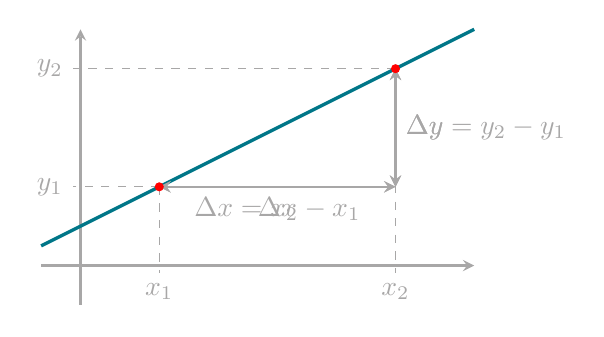
\begin{tikzpicture}[pfeil]

    % \draw[thick, fill=petrol!20, draw=petrol-lighter, rounded corners=2ex, opacity=0.5] (0,0) rectangle ++ (1.5,3.5);
    % \draw[thick, fill=darkgoldenrod!20, draw=darkgoldenrod-lighter, rounded corners=2ex, opacity=0.5] (5,0) rectangle ++ (1.5,3.5);

    \draw[stealth-stealth, thick,white] (4,1)-- node[right] {$\Delta y=y_2-y_1$} (4,2.5);
			
    \draw[thick, -stealth] (-0.5,0) -- (5,0);
    \draw[thick, -stealth] (0,-0.5) -- (0,3);
    
    \draw[very thick, petrol] (-0.5,0.25) -- (5,3);
    
    
    
    \draw[dashed] (1,1) -- (1,-0.1) node[below]{$x_1$};
    \draw[dashed] (4,2.5) -- (4,-0.1) node[below]{$x_2$};
    \draw[stealth-stealth, thick] (1,1)-- node[below] {$\Delta x$} (4,1);
    \draw[stealth-stealth, thick] (1,1)-- node[below] {$\Delta x=x_2-x_1$} (4,1);
    
    \draw[dashed] (1,1) -- (-0.1,1) node[left] {$y_1$};
    \draw[dashed] (4,2.5) -- (-0.1,2.5) node[left]{$y_2$};
    
    \draw[stealth-stealth, thick] (4,1)-- node[right] {$\Delta y$} (4,2.5);
    \draw[stealth-stealth, thick] (4,1)-- node[right] {$\Delta y=y_2-y_1$} (4,2.5);
    
    
    \draw[red,fill] (1,1) circle (0.05);
    \draw[red,fill] (4,2.5) circle (0.05);
    

\end{tikzpicture}

\end{document}
